\chapter{Power}
\label{ch:Power}
An effective mission analysis is crucial to estimating the power required to operate the \textit{Swing} over the whole mission profile; hence, this chapter heavily builds upon the findings of \Cref{ch:Mission_Profile}.

\section{Power Required Model}
\label{subsec:powermodel}
The model presented in \Cref{eq:powermodel} is used to estimate the power required by the \textit{Swing} to operate nominally \cite{helicoptercourseMarilena}, as established in \Cref{ch:Mission_Profile}.
Where $P_{\text{req}}$ is the total required power, $P_{\text{p}}$ the profile power, $P_{\text{i}}$ the induced power and lastly, $P_{\text{par}}$ is the parasite power. Such power components are explained in detail in the following paragraphs.
\begin{equation}
\label{eq:powermodel}
    P_{\text{req}}=P_{\text{p}}+P_{\text{i}}+P_{\text{par}}
\end{equation}

\subsubsection{Profile Power} 
It incorporates the power required to overcome the profile drag of the rotor blades and wings (lifting surfaces), inherently due to their aerodynamic shape and skin friction, as they move through the air \cite{helicoptercourseMarilena}.
It is calculated as shown in \Cref{eq:profilepower}. 
With $\sigma$ being the solidity of a single rotor, $\rho$ the density of air, $\Omega$ the rotor rotational velocity in \unit{rad\per\s}, $V$ the horizontal velocity in \unit{m\per\s}, and $R$ the rotor radius in \unit{m}.
Lastly, multiplication by $N_{\text{eng}}$ is needed to compute the total profile power of the vehicle. $\bar{C}_{Dp}$ is the coefficient of rotor profile drag determined by empirical, rotor-specific relations \cite{HelicopterFlight}.
Normally contributing thinly to the total required power during flight, the profile power increases with increasing vehicle horizontal speed. 

\begin{equation}
\label{eq:profilepower}
    P_p=N_{\text{eng}}\cdot\frac{\sigma \bar{C}_{Dp}}{8} \rho(\Omega R)^3 \pi R^2\left(1+4.65 \mu^2\right),\quad\text{with }\mu=\frac{V}{\Omega R}
\end{equation}


\subsubsection{Induced Power} 
It represents the power required to overcome induced drag in an aircraft, particularly significant in vertical flight (in which very high rotor-induced velocities are generated).
Induced drag is the aerodynamic resistance generated as a byproduct of lift creation~\cite{helicoptercourseMarilena}.
\Cref{eq:inducedPower} is the formulation of induced power used in the present model.
Where $k$ is a factor ranging from 1.1 to 1.2, $T$ is the total thrust required by the vehicle at a specific moment, and $v_i$ the velocity induced by each rotor, which can be computed as $v_i=\bar{v_i}\cdot \sqrt{\frac{W}{2N_{\text{eng}}\rho \pi R^2}}$.
The parameter $\bar{v_i}$ can be found numerically by computing the roots of \Cref{eq:vibar}, valid for low horizontal speeds~\cite{helicoptercourseMarilena}.
Induced drag is, therefore, inversely proportional to the square of the airspeed. Moreover, as high thrust settings are experienced during the first stages of transition (low horizontal velocity), even higher induced power levels are expected at lower speeds, decreasing significantly at higher speeds.

\begin{equation}
\label{eq:inducedPower}
    P_{\text{i}}=kTv_i
\end{equation}

\begin{equation}
\label{eq:vibar}
\bar{v_i}^4+\bar{V}^2\bar{v_i}^2-1=0,\quad\text{with }\bar{V}=\frac{\text{horizontal speed}}{\sqrt{\frac{W}{2\rho \pi R^2}}}
\end{equation}

\subsubsection{Parasite Power}
Lastly, it is the power required to overcome aerodynamic resistance generated by the aircraft’s non-lifting surfaces and components moving through the air is required.
It can be accurately computed per each horizontal velocity thanks to the aerodynamic model from \Cref{sec:AeroBuildup}, following from \Cref{eq:parasitePower}.
With $A_{\text{par, i}}$ being the parasite drag areas of each non-lifting element of the vehicle.
From \Cref{eq:parasitePower}, it can be derived that $P_{\text{par}}$ will swiftly increase with the cube of the horizontal velocity.

\begin{equation}
\label{eq:parasitePower}
    P_{\text{par}}=\Sigma A_{\text{par, i}}\frac{1}{2}\rho V^3
\end{equation}

\section{Mission Power Curve}\label{sec:missionpowercurve}
\Cref{tab:powermodelparameters} summarises the parameters determined in the previous chapters, which are inputted into the power model described in \Cref{subsec:powermodel}. The result is a plot of power required over horizontal speed, as shown in \Cref{fig:pcurveNOoptimisation}.

\begin{table}[htpb]
\centering
\caption{Parameters used for the power model}
\label{tab:powermodelparameters}
\begin{tabular}{llllllll}
    \hline
$R$ [\unit{m}] & $\Omega$ [\unit{rad/s}] & $W$ [\unit{N}] & RPM [\unit{{-}}] & $\sigma$ [\unit{{-}}] & $k$ [\unit{{-}}] & $A_{\text{par, tot}}$ [\unit{m^2}] & $T$ [\unit{N}]   \\ \midrule
   1.05 &              163\footnotemark[1] &   16200 &      1560 &           0.28 &     1.1 & Simulated                          & Simulated \\

    \bottomrule
\end{tabular}
\end{table}
\footnotetext[1]{For a conservative power estimate, $\Omega$ is taken equal to the rotational rate associated with 1300RPM, the highest RPM setting the \textit{Swing} is designed for}
\begin{figure}[htpb]
    \centering
    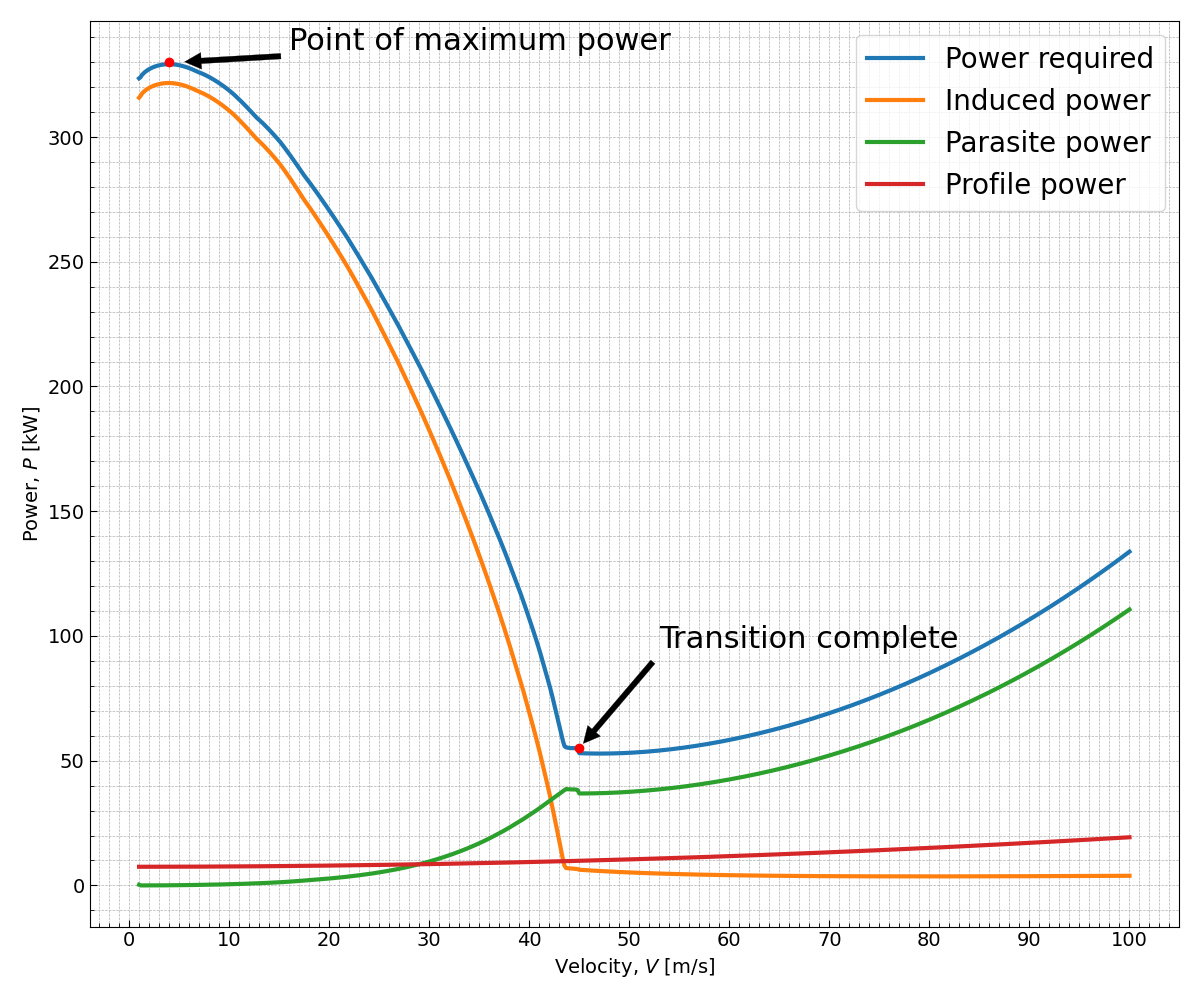
\includegraphics[width=0.7\linewidth]{figures/Propulsion/pcurveNONopt}
    \caption{Power required over velocity profile.}
    \label{fig:pcurveNOoptimisation}
\end{figure}

Several observations can be made from \Cref{fig:pcurveNOoptimisation}. 
First and foremost, as an inherent form of validation, it can be seen how the individual power contributions follow the trends predicted in \Cref{subsec:powermodel}.
The point at which transition is complete and that at which the peak of power required is estimated to occur is indicated,
respectively, at \qty{45}{m/s} and about \qty{3}{m/s}.
Interestingly, the power peak of \qty{330}{kW} is reached at a velocity of \qty{3}{m/s} (at $\sim 30\%$ of transition from vertical to horizontal flight, and not during hover, when V=\qty{0}{m/s}), likely
as a consequence of the extra thrust required to be delivered by the engines to compensate for a loss in lift caused by the inclination of the thrust line.
The thrust required to keep vertical equilibrium during the transition,
causing very high values of induced power, mainly depending on the transition stage (or transition value);
extensive discussion on this can be found in \Cref{subsec:transition}.
Hereafter, the power required swiftly decreases to match standard horizontal flight conditions at \qty{45}{m/s}.
Being the cruise speed of about \qty{56}{m/s} (\qty{200}{km/h}),
the required power is expected to stay well within \qty{60}{kW} at all times during cruise,
making the aircraft very efficient in horizontal flight \cite{kadhiresan2019conceptualevtol}.
